\section{Optimization}
In the following, we present the methods we used to gradually improve the
performance of the algorithm. We name the different implementations that we
obtained according to the methods we employed.  \autoref{fig:DecTree} gives
an overview of the optimizations applied.

\begin{figure}[htb]

\begin{center}
\begin{tikzpicture}[-,shorten >=1pt,auto,node distance=1.8cm,
  thick,main node/.style={font=\sffamily\scriptsize\bfseries}]
	
  \node[main node] (0) {Baseline};
  \node[main node] (1) [below=1em of 0] {Transposed};
	\node[main node] (2) [below=1em of 1] {Bottom-Up};
	\node[main node] (3) [below=1em of 2] {Partial-Results};
	\node[main node] (4) [below left=1em and 1em of 3] {Triangular};
	\node[main node] (5) [below=1em of 4] {Vectorized, Triangular};
	\node[main node] (6) [below right=1em and 1em of 3] {Blocking};
	\node[main node] (7) [below=1em of 6] {Vectorized, Blocking};

  \path[every node/.style={font=\sffamily\small}]
	(0) edge node [below] {} (1)
	  (1) edge node [below] {} (2)
		(2) edge node [below] {}(3)
		(3) edge node [below] {}(4)
		(4) edge node [below] {}(5)
		(3) edge node [below] {}(6)
		(6) edge node [below] {}(7)
		;
\end{tikzpicture}
\end{center}
\caption{Overview of optimizations.}
\label{fig:DecTree}
\end{figure}

\begin{figure}[htb]\centering
	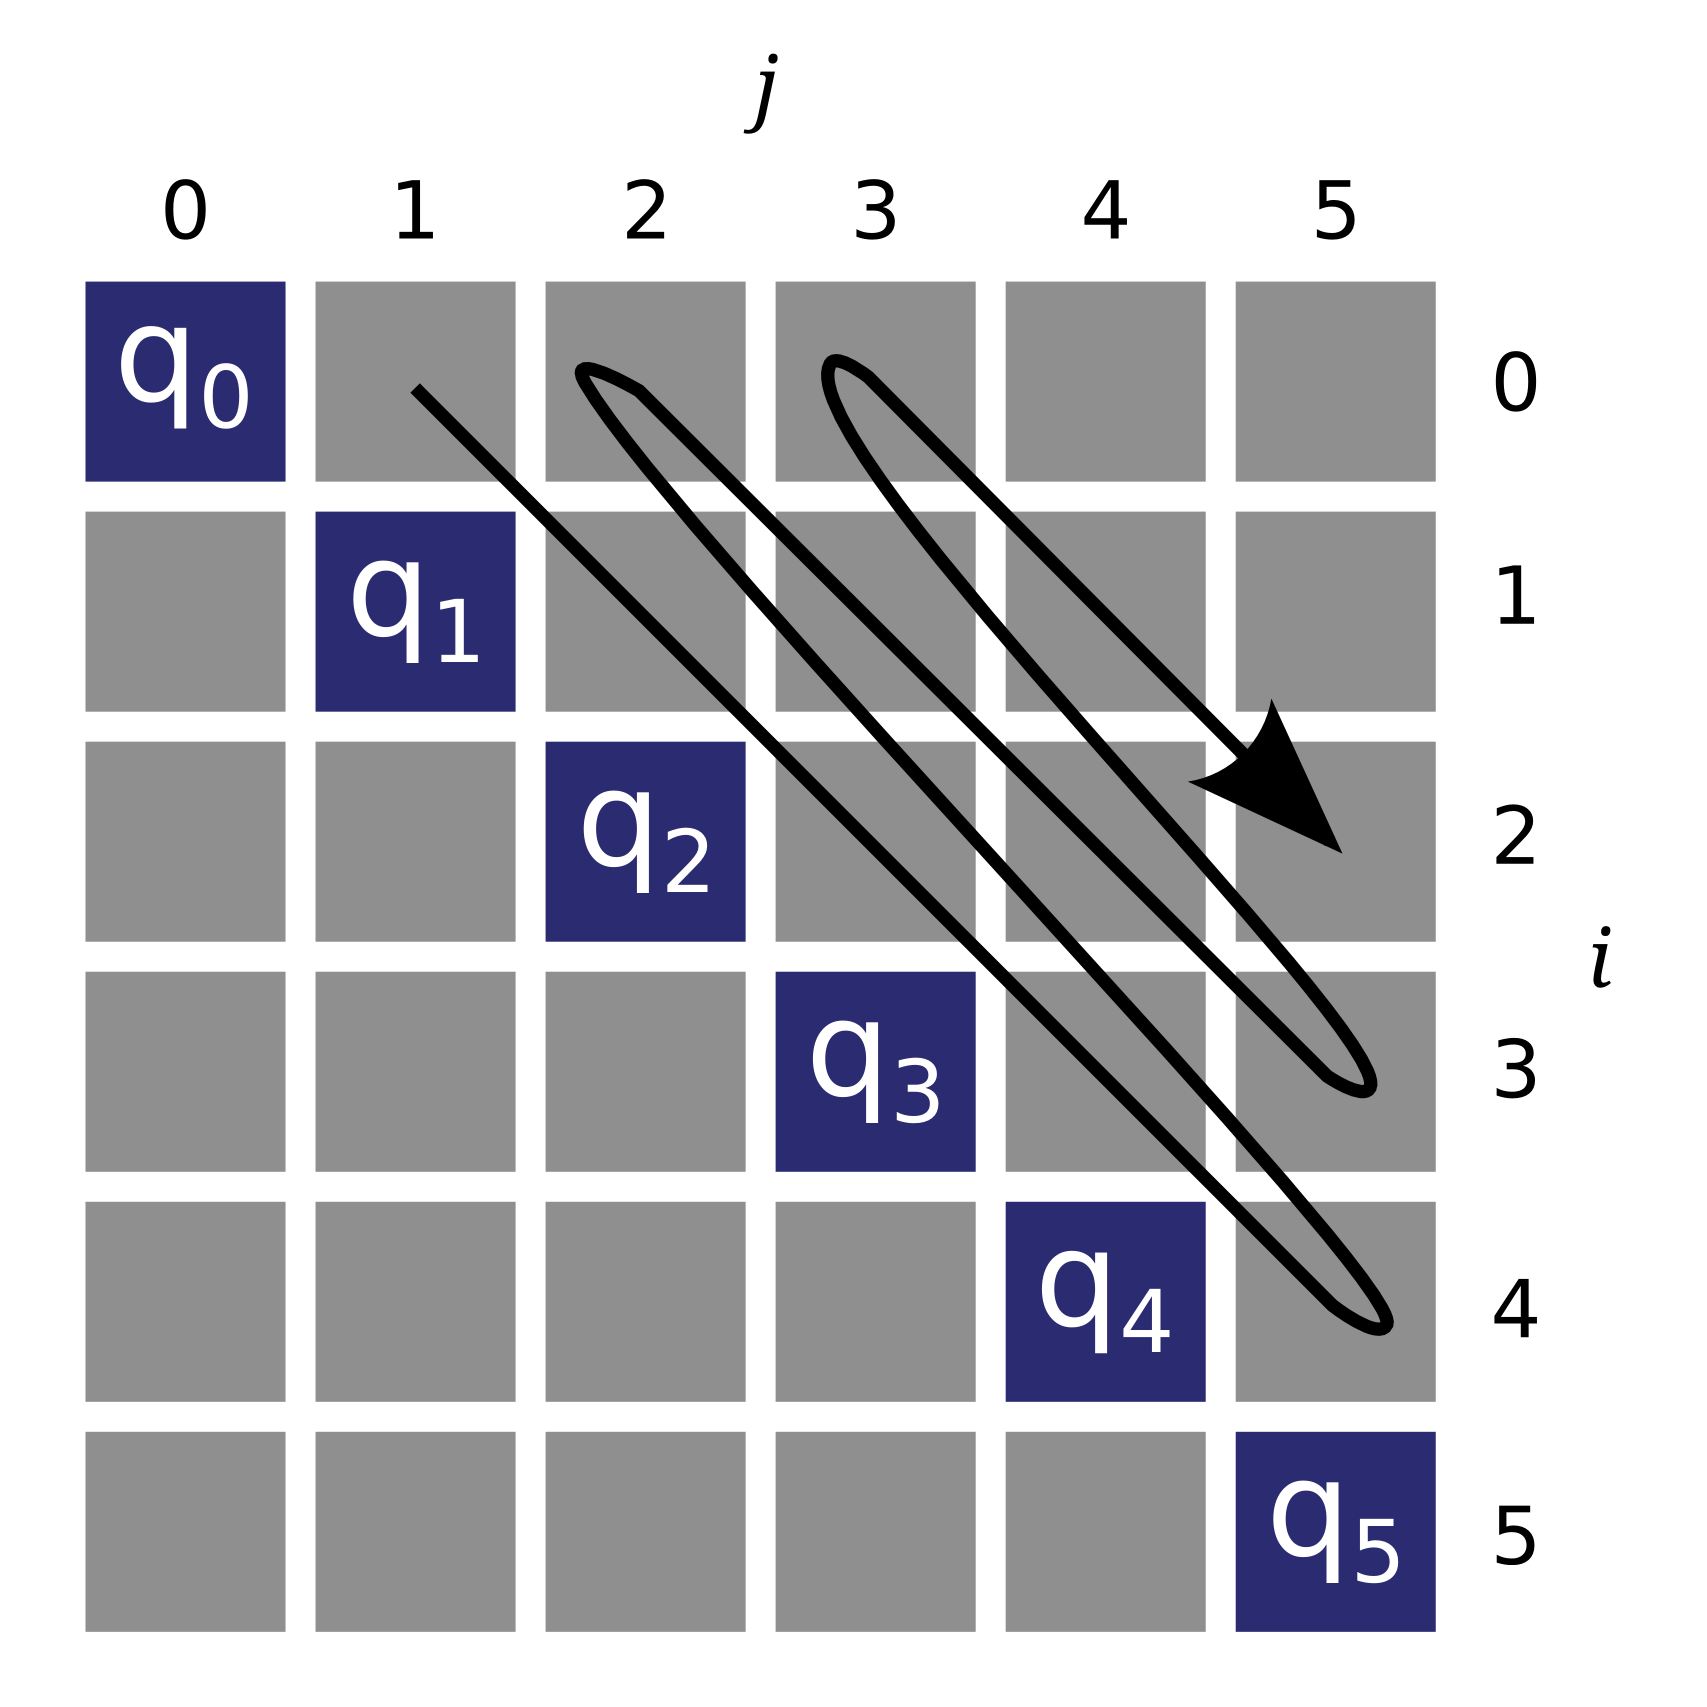
\includegraphics[width=0.33\textwidth]{img/reference_access.png}
  \caption{Access Pattern of reference implementation.\label{fig:reference}}
\end{figure}

\mypar{Transposed} Examining the innermost loop, we see that the table is
accessed row- and column-wise. Thus, the memory is accessed in strides of $1$
and $n+1$, respectively. However, with two simple changes to the algorithm, we
can avoid strides of $n+1$ and replace them with accesses of stride $1$: We make
use of the lower half of the square table in that we store newly calculated
values not only at $(i,j)$ but also at $(j,i)$. That is, instead of accessing a
column in the upper half, we access a row in the lower-half. This needs only two
minor changes to the algorithm as described in \autoref{lst:baseline}:
First, line $7$ turns into
\begin{center}
\verb:t = e[IDX(i,r)] + e[IDX(j,r+1)]:, 
\end{center}
and after line $10$, we would insert 
\begin{center}
	\verb:e[IDX(j,i)] = t;:.
\end{center}

\mypar{Bottom-Up} The order in which individual values are calculated is
along the diagonals, as visualized in Figure \ref{fig:reference}. We notice
that, for two distinct cells on a diagonal, their corresponding rows and
columns intersect exactly in one cell. By changing the outermost two loops
determining the target cell such that the table is built up row-wise and
bottom-up, as visualized in Figure \ref{fig:bottom-up}, we can improve
temporal locality with respect to the accesses to the row that is currently
being built-up.

\begin{figure}[htb]\centering
	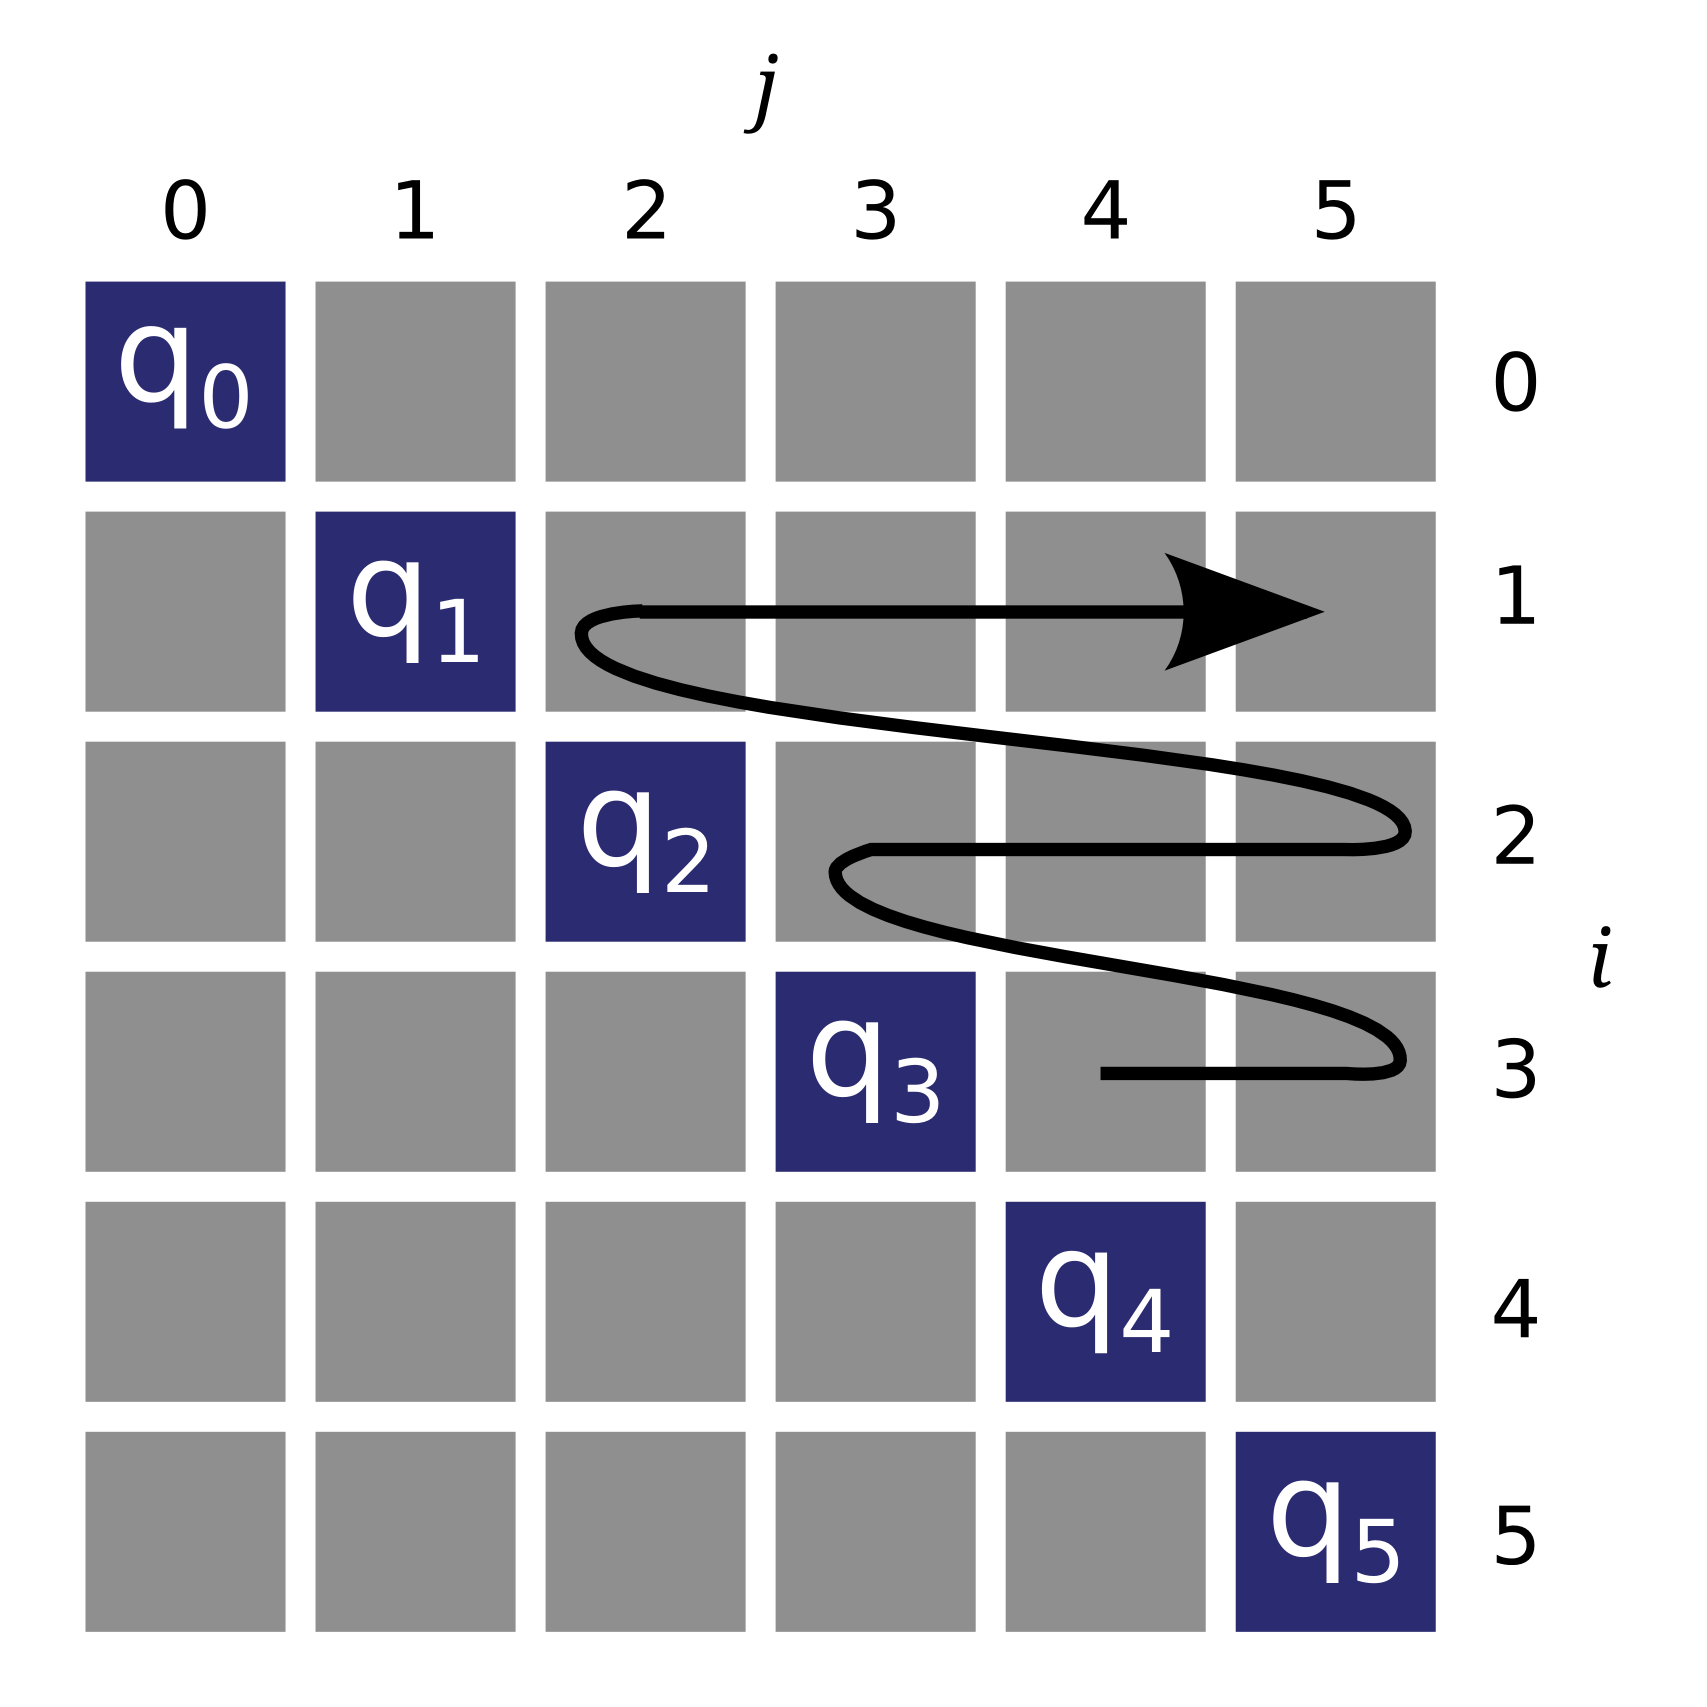
\includegraphics[width=0.33\textwidth]{img/bottom_up_access.png}
  \caption{Access Pattern of Bottom-Up.\label{fig:bottom-up}}
\end{figure}

\mypar{Partial Results} Instead of calculating the minimum value over a full row
and column, we can store intermediate values for an entire row by swapping the
innermost two loops. That is, for row $i$, we add the value $e[i,r], i\leq r\leq
n$ to all entries $e[r,j], r\leq j \leq n$ and store the minimum of that sum and
$e[i,r]$ in $e[i,r]$. \autoref{fig:partial} visualizes the pattern for one
consecutive executions of the $r$-loop (which is now the second innermost loop):
the value contained in the cell with the unfilled circle is added to all values
contained in the cells with the filled circle and the minimum is stored in the
white cells. This allows to have sequential access in the innermost loop
without the need to keep the transposed version of the data values in the
lower left half of the triangle.

\begin{figure}[htb]\centering
	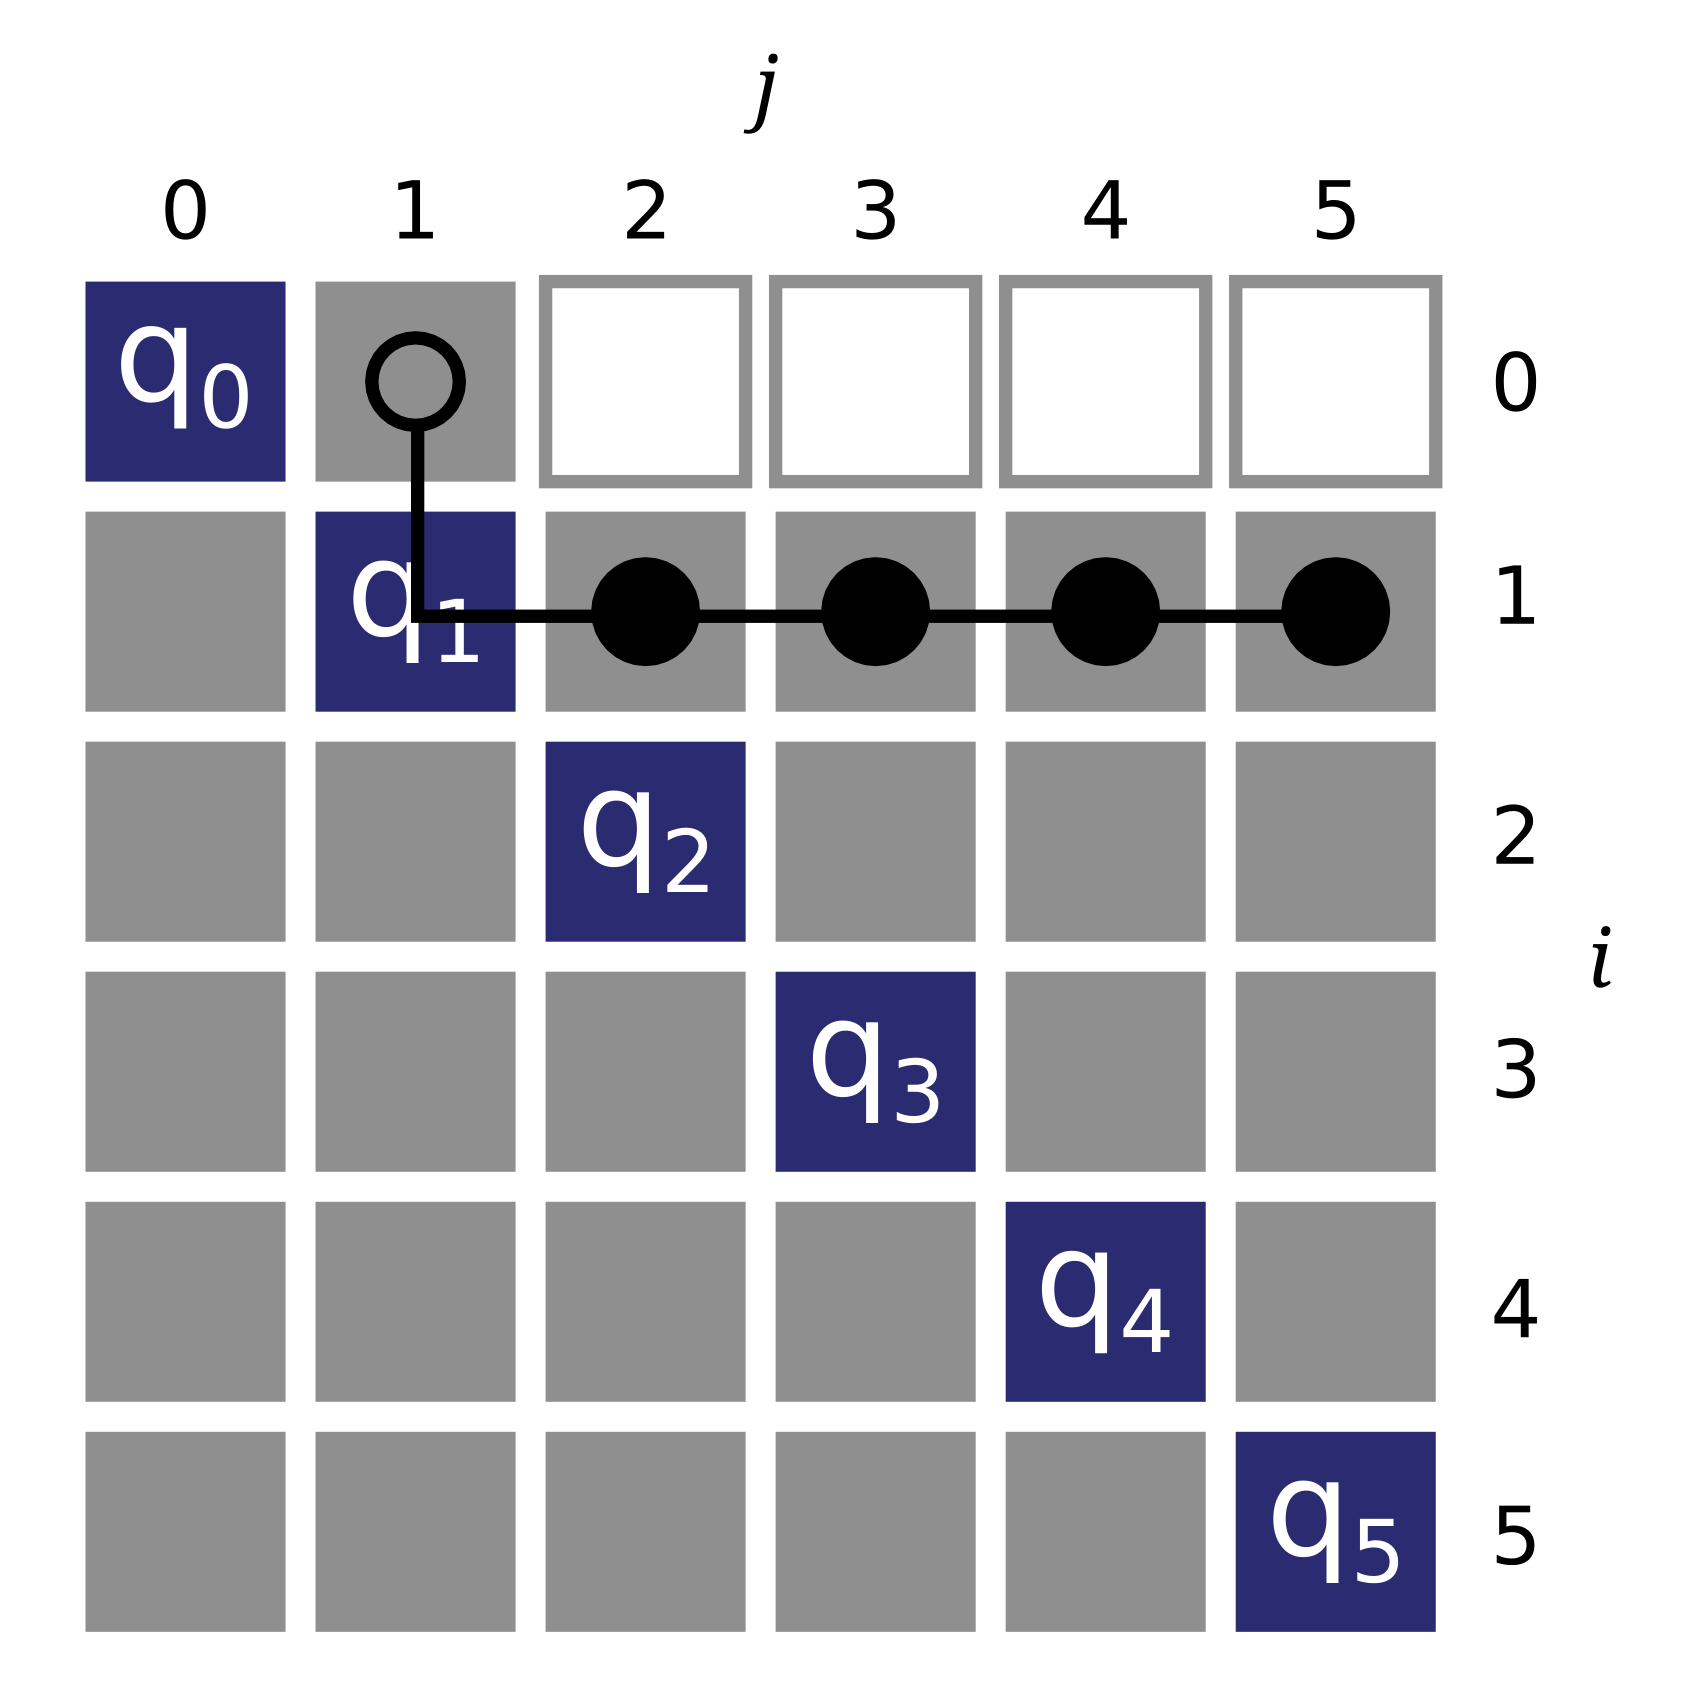
\includegraphics[width=0.33\textwidth]{img/intermediate_access.png}
  \caption{Storing Partial results.\label{fig:partial}}
\end{figure}

\mypar{Triangular} While the above approach need not necessarily improve
the performance over the \emph{Bottom Up}-approach, allocating the full
square memory is no longer required. We can \emph{compress} the memory
layout by concatenating the rows of the ``upper'' triangular table.  As for
each target row $i$ we compute, the full triangle below it is accessed row
after row, this yields unit stride access even at the end of each
intermediate row being traversed. The unused sections between the left end
of the square and the beginning of the triangle is now omitted. This
potentially also improves the performance of the hardware prefetcher. We
call this memory layout \emph{triangular}--as opposed to the \emph{square}
layout.

Using this memory layout significantly complicates the index calculation.
The correct index-macro for this memory layout is:
\begin{center}
	\scriptsize
	\begin{verbatim}#define IDX(i,j)\
	((n+1)*(n+2)/2 - (n-(i)+1)*(n-(i)+2)/2 + (j) - (i))\end{verbatim}
\end{center}
Strength reduction can be applied to alleviate the computation. Index
variables with constant offset changes over loop iterations make the
involved index computation obsolete.

\mypar{Vectorized Triangular} Historically, our initial approaches at
blocking, explained below, were unsuccessful. Thus, we focused on
vectorizing the triangular layout, which is straight-forward: The current
row is processed until the number of remaining cells is a multiple of the
vector length. From then on, vector instructions are used.

\mypar{Blocking} Based upon our \emph{Partial Results} approach, we employed a
blocking strategy as follows: We unrolled the two innermost loops.
Thus, instead of storing the partial results in the target row for each
subsequent row, we store calculate the minimum across multiple subsequent rows
before storing the result.
Figure \ref{fig:vec-blocking} visualizes the approach: The value stored in the
cell with the unfilled circle is added to the corresponding values stored in the
cells containing the filled circles. The minimum across the columns containing
the filled circles is stored in the empty cells which therefore contain partial
results.

\begin{figure}[htb]\centering
	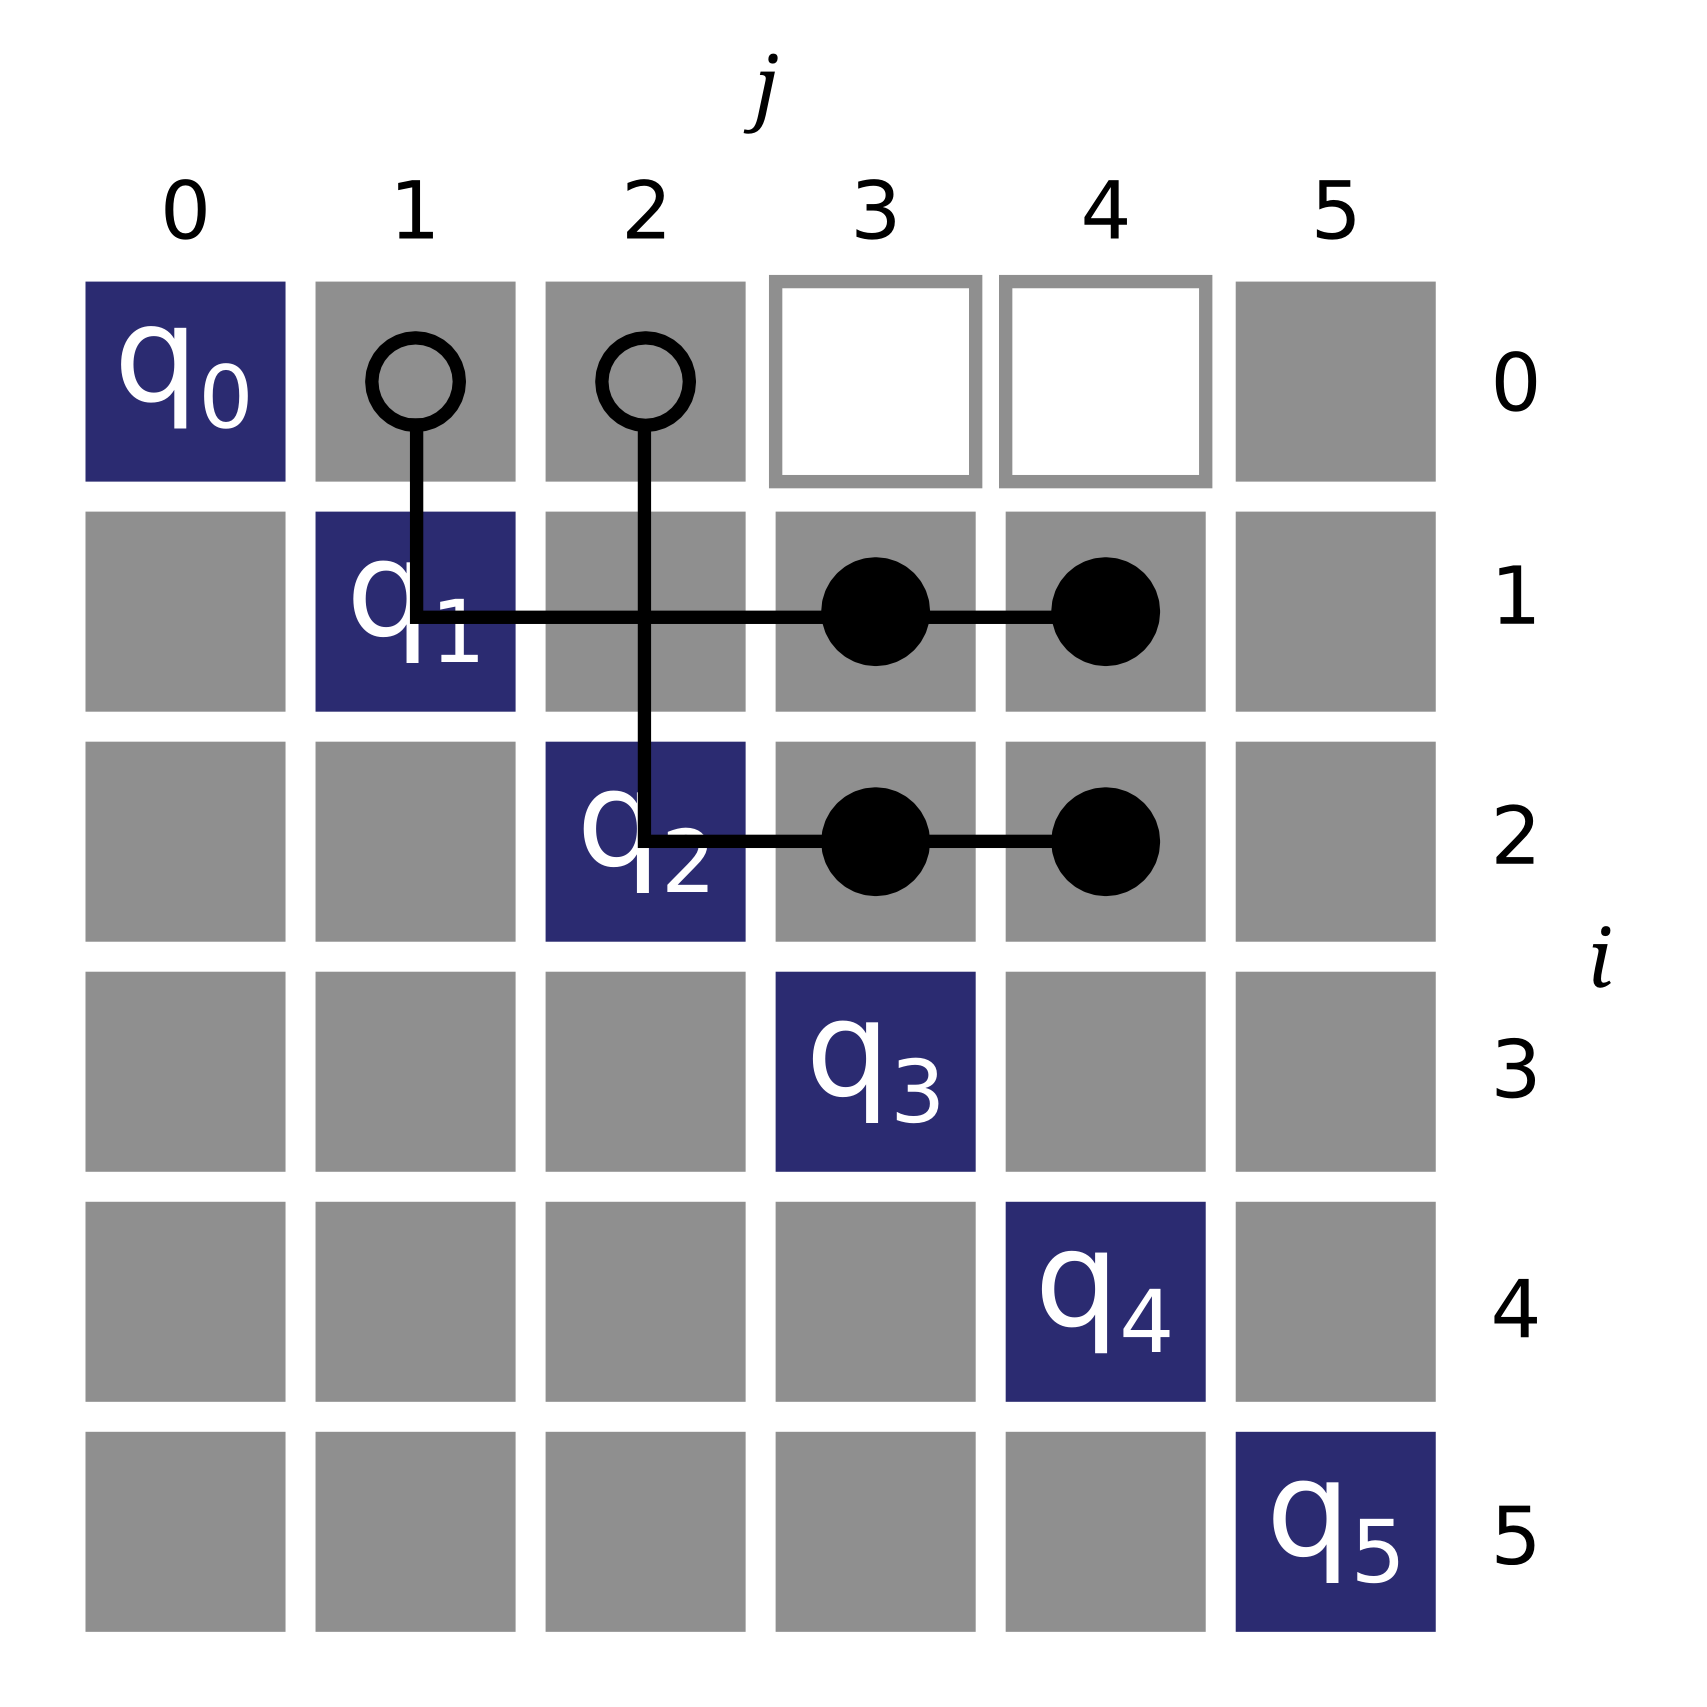
\includegraphics[width=0.33\textwidth]{img/vectorized_blocking.png}
  \caption{Vectorization of Partial Results.\label{fig:vec-blocking}}
\end{figure}

\mypar{Vectorized Blocking} Once we properly implemented blocking, it is
straight-forward to apply vectorization.
